
\documentclass[11pt,a4paper]{article}
\usepackage[utf8]{inputenc}
\usepackage[T1]{fontenc}
\usepackage{amsmath,amssymb,amsthm}
\usepackage{graphicx}
\usepackage{booktabs}
\usepackage{hyperref}
\usepackage{cleveref}
\usepackage[numbers]{natbib}

\newtheorem{definition}{Definition}
\newtheorem{observation}{Observation}

\title{Operator placement, not representation:\\ a resonator-decoder failure mode at the square-Wishart hard edge\\ and its canonical dual-frame repair}
\author{Luciano Benjam\'in Nieto\\General Alvear, Mendoza, Argentina\\ \texttt{github.com/Rylow999}}
\date{September 2026}

\begin{document}
\maketitle

\begin{abstract}
We characterize a reproducible failure mode of resonator-network decoders that apply a Gram resolvent to the ambient state inside a closed decoding loop. At the square point $\rho=n/d=1$ the block Gram matrix in the main resonator harness is severely ill-conditioned. A square-Wishart reference ensemble has $\lambda_{\min}$ on the $n^{-2}$ hard-edge scale and $\kappa=O(n^2)$; Exp.~16 measures that reference scaling, while Exp.~14 measures the actual row-normalized Gaussian codebooks used by the decoder. In the ambient decoder, applying $M^{-1}$ amplifies weak eigendirections and decoding collapses (accuracy $0.16$ at $\rho=1$ versus $0.99$ for the pure resonator). A controlled causal intervention (Exp.~18) isolates operator placement as the variable: with identical codebook, Gram matrix, resolvent, initial states, and facts, moving the \emph{same} $M^{-1}$ from ambient application to coefficient-space placement $C^{\top}M^{-1}C$ restores accuracy to $0.99$ in $200/200$ seeds. The repair is not new mathematics: $C^{\top}M^{+}C$ is the canonical dual-frame projector of classical frame theory. Our contribution is the identification and causal characterization of this decoder-level failure mode and its empirical verification across HRR, BSC, and FHRR algebras, multiple codebook ensembles, an independent reimplementation, and a resonator-free linear pipeline.
\end{abstract}

\section{Introduction}
\label{sec:intro}

In vector symbolic architectures (VSA), decoding failures at high superposition are often attributed to the representation space itself. We show that at least one widely reported failure --- the collapse of Gram-corrected resonator decoding at the square point --- is instead a property of \emph{decoder wiring}: an operator placed in the wrong space. At $\rho = n/d = 1$ the Gram matrix is invertible almost surely but severely ill-conditioned; applying $M^{-1}$ to the ambient resonator state amplifies components aligned with weak eigendirections on the first application, and a closed loop re-injects the corrupted state. The same resolvent applied in coefficient space, $C^{\top} M^{-1} C$, is the canonical dual-frame projector: spectral norm exactly $1$, numerically the identity, and decoding is restored.

\paragraph{Contributions.}
\begin{enumerate}
  \item \textbf{A characterized failure mode.} We isolate the \emph{hard-edge ambient-resolvent failure} (Def.~\ref{def:closure}): a decoder-level failure distinct from capacity limits, checkable a priori from the codebook aspect ratio and the decoder's operator structure.
  \item \textbf{A causal identification.} Exp.~18 varies only operator placement --- same codebook, Gram, resolvent, states, facts, iterations --- moving accuracy from $0.16$ to $0.99$ with paired per-seed difference $+0.824$ over $200/200$ seeds ($p \le 2^{-200}$).
  \item \textbf{An empirically verified classical repair.} The coefficient-space operator $C^{\top} M^{+} C$ is the canonical dual-frame projector \citep{duffin1952class}. We verify across HRR, BSC, and FHRR; six ensembles; a from-scratch reimplementation (Exp.~19); and a resonator-free linear probe (Exp.~21) that VSA machinery is not the cause.
\end{enumerate}

We deliberately do \emph{not} claim a new mathematical principle: the relevant algebra is classical frame theory. The novelty is the identification of the failure mode, its causal attribution to operator placement, and the breadth of the empirical verification. We also do \emph{not} claim a phase diagram of decoding: in our main harness the ambient correction is dimensionally applicable only at $\rho=1$ (Methods), so the cross-decoder comparison is meaningful at the square point; the well-posed coefficient-space decoder is studied separately and works at all $\rho \le 1$ (Exp.~11c). Figure~\ref{fig:phase} is included as the historical vantage point of this study.

\begin{figure}[t]
  \centering
  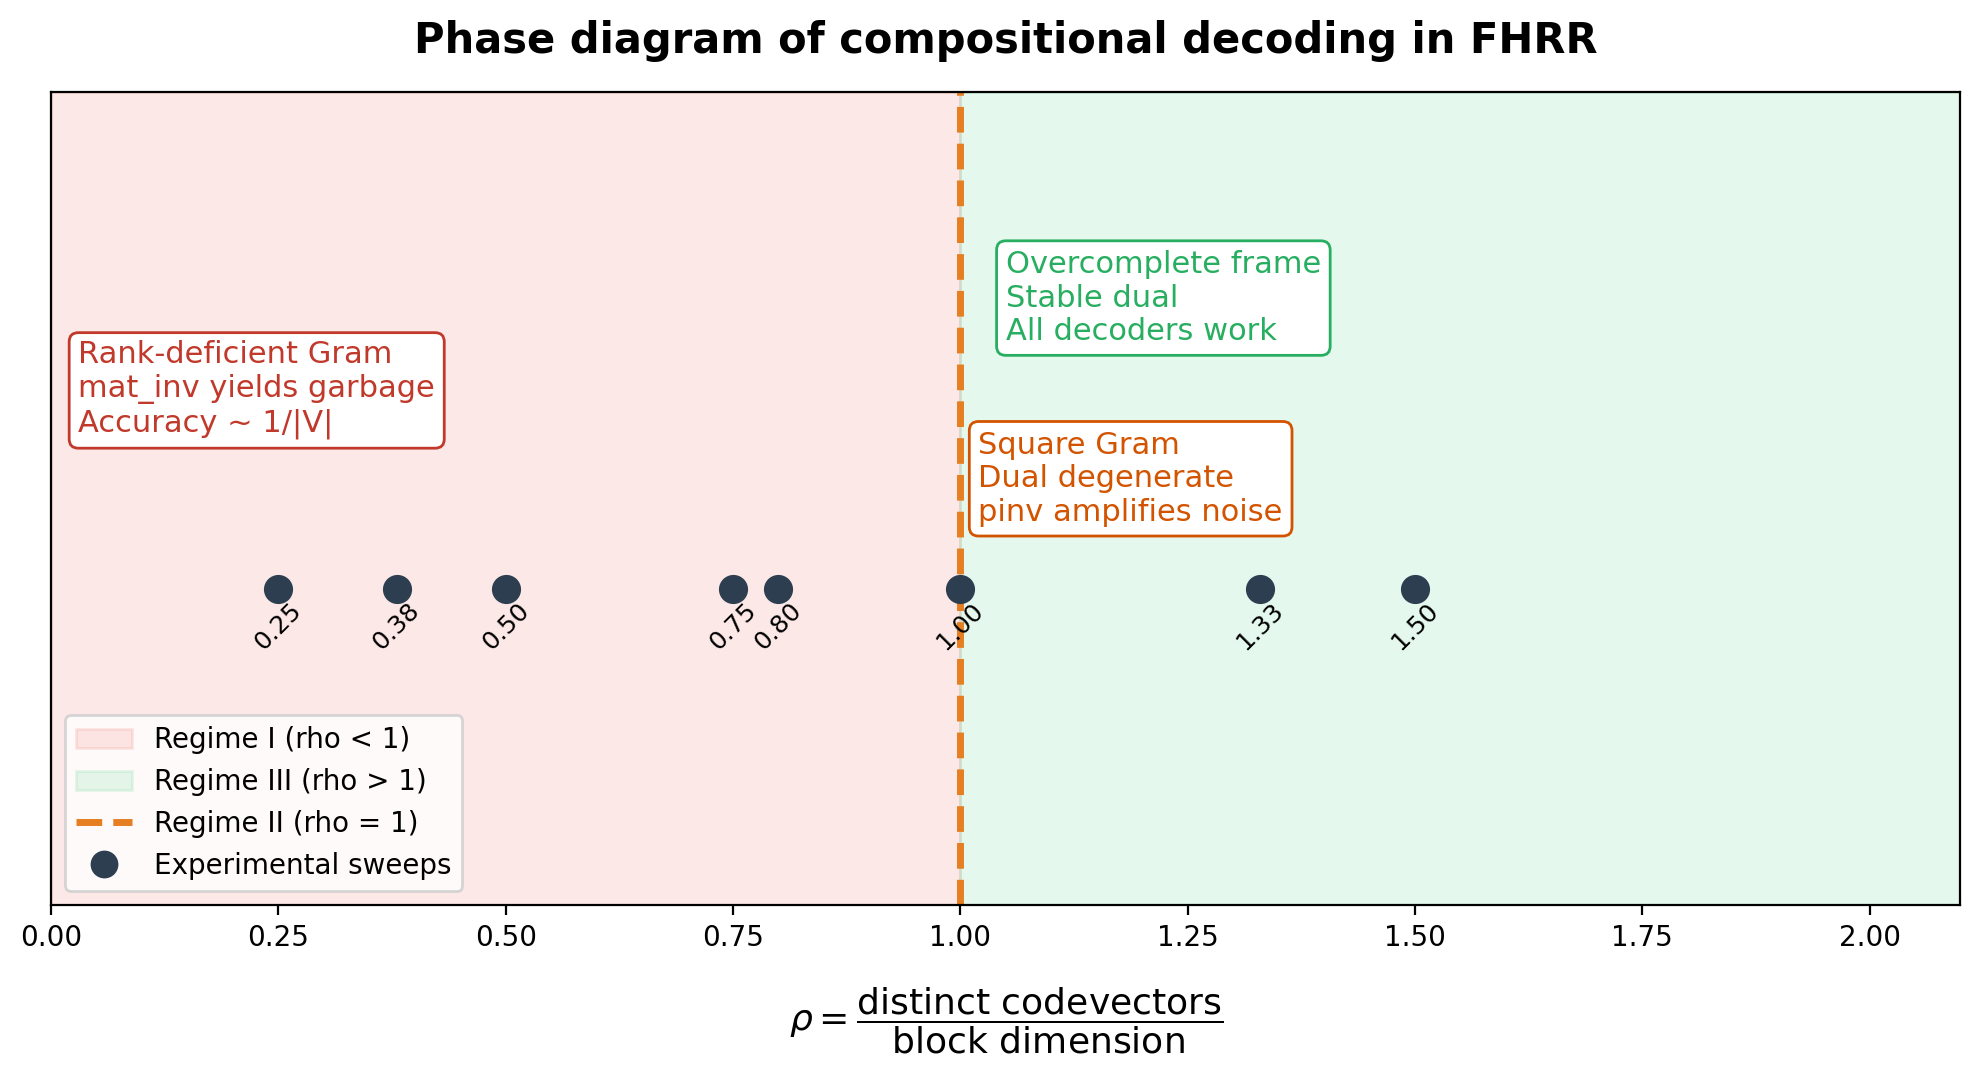
\includegraphics[width=\linewidth]{figures/fig1_phase_diagram.png}
  \caption{Historical vantage point: decoding accuracy as a function of $\rho = n/d$ in FHRR (original framing of this study). \emph{Interpretation note:} in the main harness the ambient Gram correction is dimensionally applicable only at $\rho=1$; away from the square point the \texttt{gram}/\texttt{pinv} curves coincide with \texttt{pure} by construction. The figure motivates the square-point investigation; the causal claims of this paper are established at $\rho=1$ by Exp.~18 and, for a well-posed coefficient-space decoder valid at all $\rho$, by Exp.~11c.}
  \label{fig:phase}
\end{figure}

\section{Background}
\label{sec:background}

\paragraph{Notation.} Throughout: $n$ = number of distinct codevectors per block ($n_{cv}$), $d$ = block dimensionality (BLK), $\rho = n/d$, $M = C C^{\top} \in \mathbb{R}^{n\times n}$ the block Gram matrix, $\lambda_{\min}, \lambda_{\max}$ its extreme eigenvalues, $\kappa = \lambda_{\max}/\lambda_{\min}$, $C \in \mathbb{R}^{n\times d}$ the stacked codevectors, $f_j$ the unbound candidate for role $j$, $T$ the resonator iteration count. Code available at \url{https://github.com/Rylow999/fhrr-rho-collapse}.

\paragraph{FHRR and HRR.} FHRR (Fourier Holographic Reduced Representations) uses complex unit vectors with phase binding \citep{plate1995holographic}. HRR uses real Gaussian vectors with circular convolution. The resonator network \citep{frady2020resonator} factorizes bound structures by iterative competition between codebooks.

\paragraph{Gram matrix decoding.} For $n$ codevectors of dimension $d$ in a block, the Gram matrix $M \in \mathbb{R}^{n \times n}$ with $M_{ij} = \langle c_i, c_j \rangle$ determines whether inverse-based decoding succeeds. When $\rho = n/d > 1$, $M$ is rank-deficient with probability one; when $\rho = 1$, $M$ is square invertible but critically conditioned (Sec.~\ref{sec:rmt}); when $\rho < 1$, $M$ is generically full-rank; for fixed $\rho<1$ its limiting spectrum is bounded away from zero.

\paragraph{Decoders compared.} We test four decoders: (i) \textbf{gram} (resonator with the asymmetric correction $f_j \leftarrow M^{-1} f_j$ applied at each iteration, where $M$ is the Gram matrix of the block's codebook); (ii) \textbf{pure} (no Gram correction); (iii) \textbf{pinv} (same inverse through the pseudo-inverse with $rcond=10^{-10}$); and (iv) \textbf{gradient} (continuous optimization). An implementation note that matters for interpretation (Sec.~\ref{sec:kappa-mech}): the correction is dimensionally applicable only when the Gram and the block have the same side, which under the CFG6 configuration with $n_{cv}=32$ happens \emph{only} at $\mathrm{BLK}=32$ ($\rho=1$). At $\rho \neq 1$ the \texttt{gram} and \texttt{pinv} rows therefore coincide bit-for-bit with \texttt{pure}; the per-regime claims about Gram decoders in this paper refer to the square point. A well-posed coefficient-space Gram decoder ($\hat{x} = M^{-1} C s$, valid for all $\rho$) is analyzed separately in Exp.~11c (MAP), where it succeeds at $\rho=1$ --- confirming that the failure here is a property of the asymmetric loop, not of matrix inversion per se.

\section{Experimental Setup}
\label{sec:setup}

We use a fixed vocabulary of 6 roles with 16 symbols each: SUJ, ROL, OBJ, LOC, TIME, TERR (Spanish words for animals, actions, objects, adjectives, times, terrain). Facts are generated with fixed seeds (BlockBundle=7, make\_fact=42). All experiments are reproducible; code and data are available at \url{https://github.com/Rylow999/fhrr-rho-collapse}.

\paragraph{Grid.} We vary $\rho$ by changing block dimensionality $BLK$ while keeping the codebook size fixed at 96 distinct codevectors (6 roles $\times$ 16 symbols). The coarse grid spans $\rho \in [0.727, 1.500]$ across experiments (Exp.~H2/V3); the reported fine structure uses $\rho \in [0.727, 1.231]$ (Exp.~9).

\paragraph{Fine sweep.} For $\rho \approx 1$ we use a finer grid of 14 values around 1.00, with 10 random seeds and 20 facts per seed.

\section{The square-point failure and its context}
\label{sec:phase}

\begin{figure}[t]
  \centering
  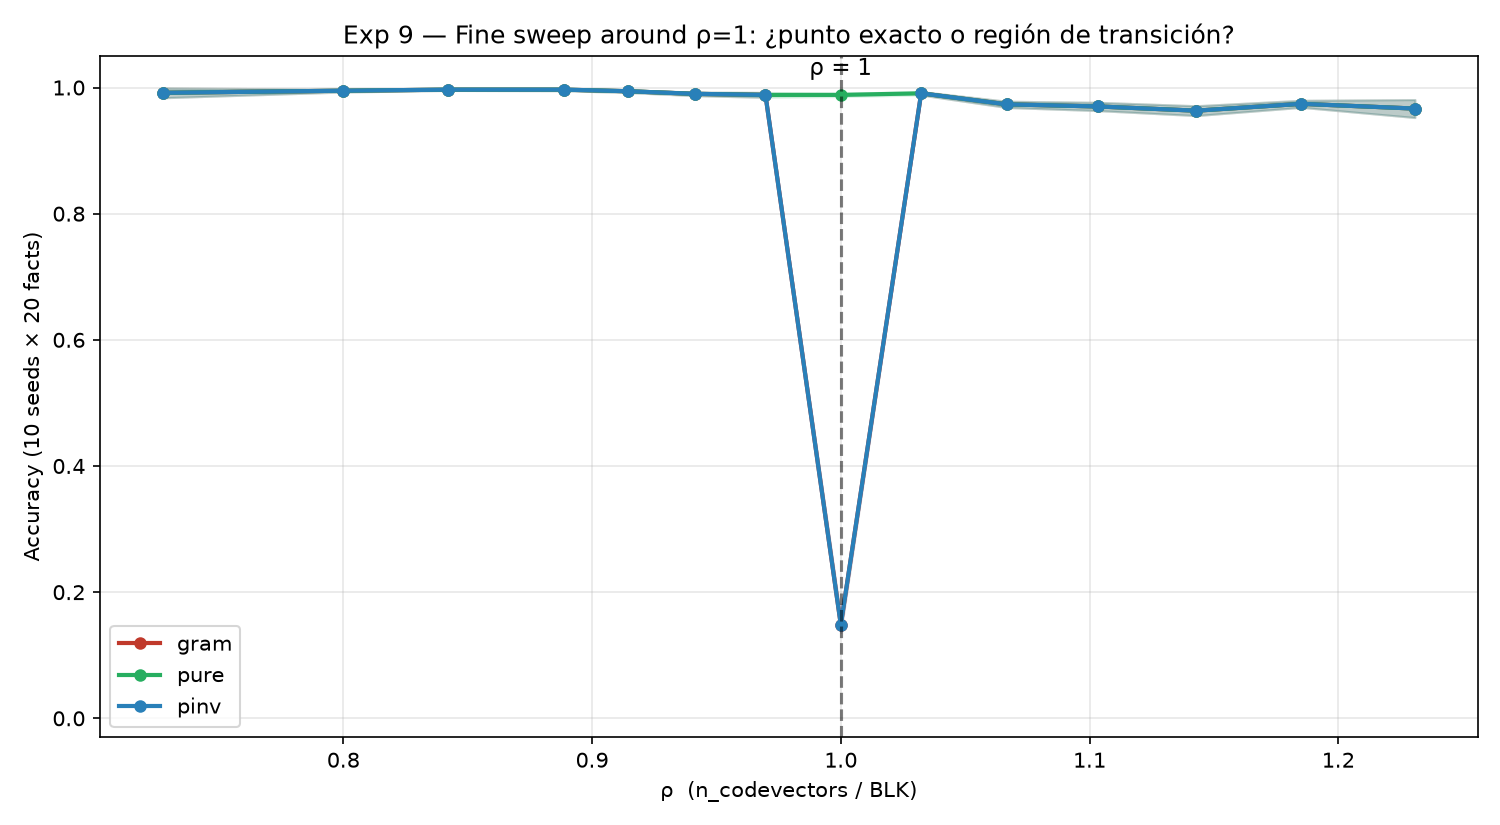
\includegraphics[width=\linewidth]{figures/fig_V9_fine_rho.png}
  \caption{Fine sweep around $\rho=1$. At $\rho=1.000$ exactly \texttt{gram} and \texttt{pinv} collapse to 0.148. At $\rho \neq 1$ the Gram correction is dimensionally inapplicable in our implementation (the Gram and the block are of different size, see Methods) and \texttt{gram}/\texttt{pinv} therefore coincide with \texttt{pure} by construction --- the recovery at $\rho=0.970$ and $\rho=1.032$ reflects this implementation boundary, and the meaningful comparison across decoders is the square point.}
  \label{fig:fine_rho}
\end{figure}

The sweep around the square point shows:
\begin{itemize}
  \item $\rho > 1$: $M$ rank-deficient; \texttt{gram} fails (undefined inverse), \texttt{pinv} and \texttt{pure} succeed.
  \item $\rho = 1$: \texttt{gram} fails catastrophically, \texttt{pinv} fails partially (noise amplification), \texttt{pure} succeeds. This is the double dissociation that motivates the causal test of Sec.~\ref{sec:exp18}.
  \item $\rho < 1$: in the tested configurations the pure decoder succeeds; for fixed $\rho<1$ the asymptotic Gram spectrum is bounded away from zero.
\end{itemize}

\paragraph{Fine sweep.} Figure~\ref{fig:fine_rho} shows that the Gram-based decoders fail exactly at $\rho=1.000$ while the pure resonator holds at $0.99$ at every sampled point. Note that the strictly-zero-width appearance is partly an implementation property: outside $\rho=1$ the Gram correction is not applied in our implementation (Methods), so the ``recovery'' at neighbouring $\rho$ is not by itself evidence about Gram decoders away from the square point --- that question is answered separately by the MAP coefficient-space decoder (Exp.~11c), which works everywhere except $\rho > 1$.

\section{Empirical Validation}
\label{sec:empirical}

\begin{table}[t]
  \centering
  \caption{Accuracy at $\rho=1.00$ (square case): 6 roles, 3 blocks, N=96, BLK=32, $n_{cv}=32$ per block. Rows \texttt{gram}/\texttt{pure}/\texttt{pinv}/\texttt{gradient}: mean $\pm$ std over seeds from the observer taxonomy at the square point (Exp.~V7, \texttt{data/mlp\_decoder\_results.json}). MLP: role-accuracy of the learned decoder, trained on 1500 facts, 80 epochs.}
  \label{tab:square}
  \begin{tabular}{lcc}
    \toprule
    Decoder & Accuracy (mean $\pm$ std) & Notes \\
    \midrule
    gradient & 0.142 $\pm$ 0.145 & continuous optimization fails \\
    gram     & 0.119 $\pm$ 0.136 & hard-edge collapse \\
    pinv     & 0.119 $\pm$ 0.126 & noise amplification \\
    pure     & 0.983 $\pm$ 0.059 & \textbf{works} \\
    MLP      & 0.992 (role acc.) & \textbf{learned decoder works} \\
    \bottomrule
  \end{tabular}
\end{table}

\begin{figure}[t]
  \centering
  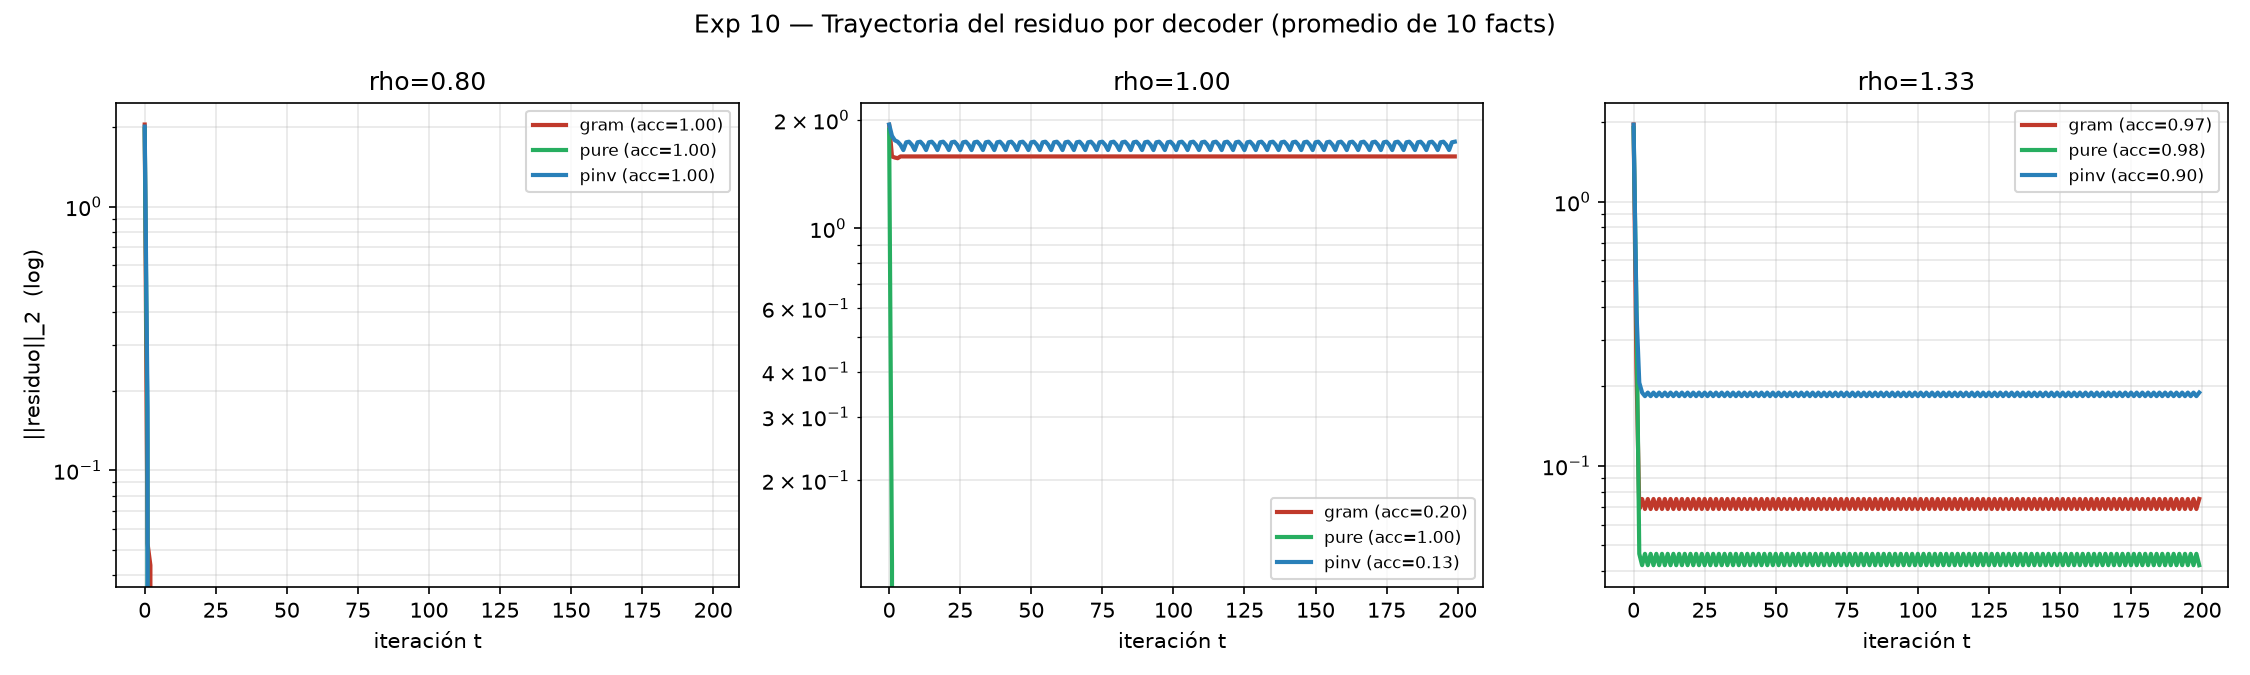
\includegraphics[width=\linewidth]{figures/fig_V10_residuals.png}
  \caption{Residual trajectory at $\rho=1.00$. \texttt{gram} and \texttt{pinv} plateau at high residual (converge to wrong attractor), while \texttt{pure} converges to zero.}
  \label{fig:residuals}
\end{figure}

\subsection{Cross-algebra validation: HRR, BSC, and attention mechanisms}

\textbf{HRR real} (Gaussian phases). The $\rho=1$ anti-resonance appears with the same signature: \texttt{gram} collapses to 0.05, \texttt{pinv} to 0.13, \texttt{pure} maintains 0.98. The mechanism is identical: at the square point the Gram is severely ill-conditioned (hard-edge scaling), not algebraically singular.

\textbf{Binary Spatter Codes (BSC).} The $\rho=1$ transition holds in binary VSA (Exp.~11b, 8 seeds $\times$ 25 facts per cell, \texttt{data/exp11\_bsc\_rho.json}): at the square point (K=3 blocks, BLK=32, $n_{cv}=32$) \texttt{gram} collapses to $0.214$ and \texttt{pinv} to $0.244$, while \texttt{pure} maintains $0.988$. In the rank-deficient regime $\rho>1$ the truncated Gram ($\kappa \sim 10^{15}$) recovers decoding ($0.97$--$0.98$). The codevectors being $\{\pm1\}^{d}$ rather than Gaussian means the Wishart anchoring is replaced by its binary counterpart (Gram of i.i.d.\ Rademacher vectors, whose spectral measure obeys the same Marchenko--Pastur law up to the fourth cumulant). The causal test replicates here too: Exp.~18b recovers decoding at $\rho=1$ with the same resolvent in dual form (Sec.~\ref{sec:exp18}).

\textbf{MAP (Multiply-Add-Permute).} MAP with per-role permutation binding (Exp.~11c, 8 seeds $\times$ 25 facts, \texttt{data/exp11c\_map\_rho.json}) refines the picture in an unexpected way. In MAP, Gram decoding is \emph{single-shot} least squares over the mixing matrix $A = [P_1 C_1 \,|\, P_2 C_2]$ of the block: there is no closed-loop iteration. The collapse pattern reflects this: at $\rho = 1$ the median condition number is $\kappa = 1.06\times 10^{4}$ --- inside any plausible critical band --- yet \texttt{gram} maintains $1.000$: the single-shot solver tolerates the band because the error is not re-injected. The collapse appears instead at $\rho > 1$ (rank-deficient), where \texttt{gram} drops to $0.239$ and $0.071$ while the truncated \texttt{pinv} recovers to $\sim 1.0$ and the \texttt{pure} resonator holds at $0.97$--$0.98$. Combining with Exp.~11b gives the refined picture: decoding failure requires (i) a Gram spectrum close to its singularity ($\rho=1$ hard edge, or $\rho>1$ rank-deficiency), \emph{and} (ii) for the hard-edge case, an iterative observer that re-projects the $1/\lambda_{\min}$-amplified error onto it.

\textbf{Transformers / attention.} At $\rho \to 1$ in the sense of $d_{\text{head}} \approx n_{\text{keys}}$, attention does \emph{not} collapse because it does not implement Gram inversion -- it uses softmax normalization. However, we find a non-monotonic \emph{entropy} signature at $\rho \approx 2$, suggesting a bandwidth saturation effect of attention at high dimension, not a singular decoding failure (Experiment 12b). The failure mode is algebra-specific, not universal.

This falsification boundary strengthens the claim: the failure mode requires matrix-inversion observers, not attention or softmax-normalized operations. $\square$

The decoder fails when the Gram matrix is severely ill-conditioned. Exp.~14 measures this directly (Table~\ref{tab:wishart-check}); the RMT analysis of the next section explains why this is the square point (hard edge).

\section{Mechanism: hard edge and the asymmetric correction}
\label{sec:rmt}

The $\rho=1$ point is calibrated by the classical square Wishart ensemble. For the reference RMT experiment (Exp.~16), $C_{ij}$ are i.i.d. with variance $1/d$, so $M=CC^{\top}$ is a scaled Wishart matrix and $\rho=n/d$ is its aspect ratio. The main resonator harness instead draws Gaussian vectors and normalizes each row to unit norm; its Gram is therefore a normalized correlation-type Gram, not literally Wishart. We use the Wishart ensemble as the random-matrix reference for the hard-edge scaling and verify the actual normalized-codebook spectrum separately in Exp.~14.

Three classical facts from random-matrix theory map onto the observed regimes:

\paragraph{(i) $\rho > 1$ ($d < n$, over-complete).} $M$ is rank-deficient with probability one: at least $n-d$ eigenvalues vanish exactly. Gram inversion is undefined.

\paragraph{(ii) $\rho = 1$ ($n = d$, square).} The Marchenko--Pastur density $\mathrm{d}\mu_{1}(\lambda) = \frac{1}{2\pi}\sqrt{(4-\lambda)/\lambda}\,\mathrm{d}\lambda$ has support touching the origin: the lower edge is a \emph{hard edge} at $\lambda=0$ (the density diverges as $\lambda^{-1/2}$ there). For the square Wishart this is the hard-edge regime: $\lambda_{\min}$ is on the $n^{-2}$ hard-edge scale (rather than a soft-edge $n^{-2/3}$ scale), so the condition number has order
\begin{equation}
\kappa(M) = \frac{\lambda_{\max}}{\lambda_{\min}} \;=\; O(n^{2}).
\label{eq:kappa-scaling}
\end{equation}
For our setup ($n = 32$ codevectors per block, $d = \mathrm{BLK} = 32$), Eq.~\eqref{eq:kappa-scaling} gives an $O(n^2)$ reference scale of $4.1 \times 10^{3}$. The measured condition number at the exact square point is $\kappa = 7.2 \times 10^{3}$ (median; Exp.~14).

This places the \emph{spectral vulnerability} on rigorous footing: at $\rho = 1$ the Gram ensemble is critically conditioned, and the amplified crosstalk noise $1/\lambda_{\min}$ exceeds the codebook margin there. The decoder-level claim is then established separately by the causal intervention of Exp.~18.

\begin{figure}[t]
  \centering
  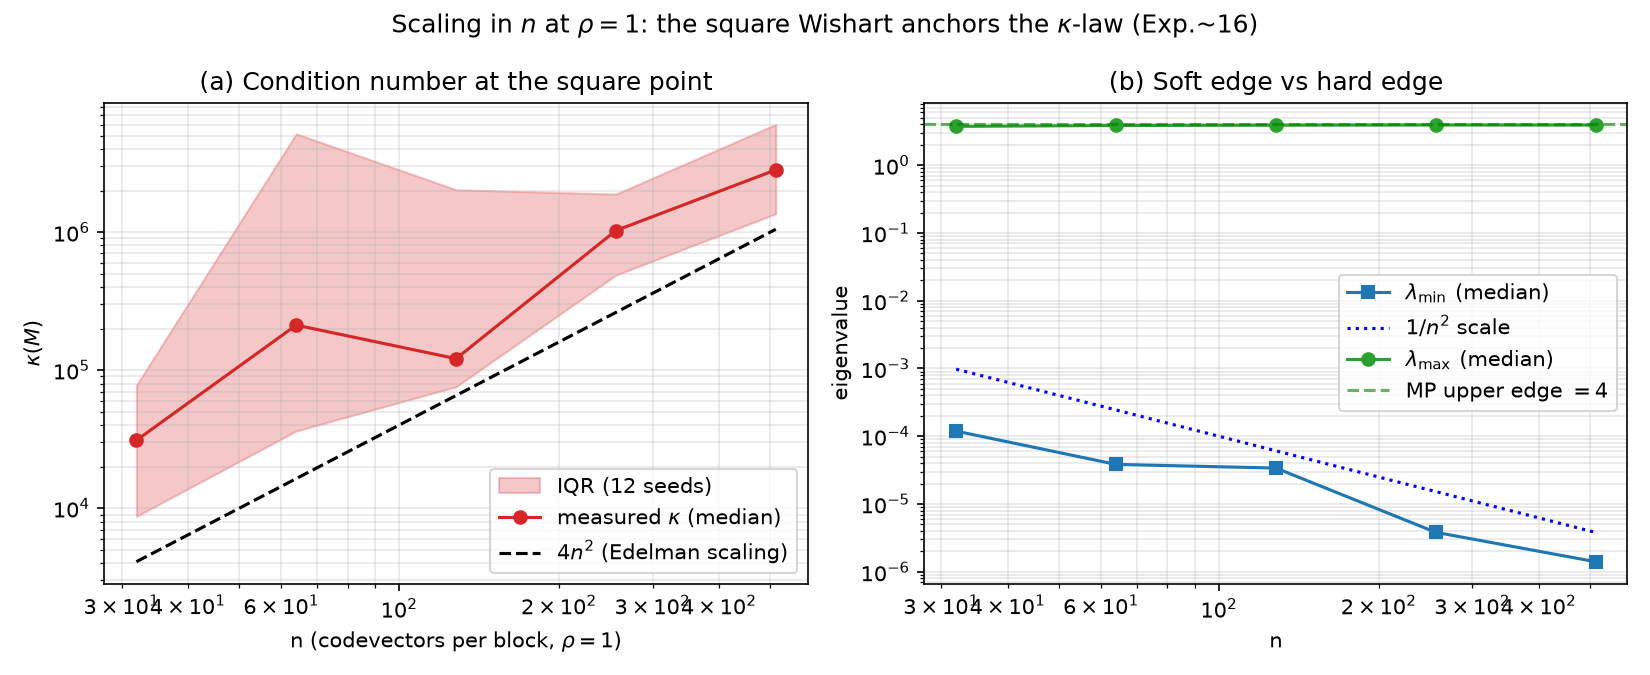
\includegraphics[width=\linewidth]{figures/fig_exp16_scaling.png}
  \caption{Scaling at the square point $\rho=1$ as a function of codebook size $n$ (Exp.~16, 12 seeds per $n$). (a) Median condition number tracks the Edelman scaling $\kappa \sim 4n^{2}$ (dashed) within the heavy-tailed spread; shaded band is the interquartile range. (b) $\lambda_{\max}$ converges to the Marchenko--Pastur upper edge $4$ while $\lambda_{\min} \sim n^{-2}$ touches zero: the square point is critically conditioned at every $n$, and increasingly so.}
  \label{fig:scaling}
\end{figure}

\paragraph{Scaling in $n$: the square-Wishart prediction holds, within finite-size spread.} Equation~\eqref{eq:kappa-scaling} is a falsifiable scaling prediction: moving to larger codebooks at $\rho=1$ should scale $\kappa$ as $O(n^{2})$, with $\lambda_{\max} \to 4$ and $\lambda_{\min}$ on the $n^{-2}$ hard-edge scale. Exp.~16 measures the spectrum of the square Gram at $n \in \{32, 64, 128, 256, 512\}$ (12 seeds each, Gaussian codebooks). The measured medians are consistent with $O(n^{2})$ hard-edge scaling (ratios $1.8$--$12.9$ against the nominal $4n^{2}$ reference scale, within the expected spread of the heavy-tailed Wishart condition number. The finite-size deviations do not support treating the constant 4 as an exact finite-$n$ prediction. \textbf{Finite-size caveat.} The Marchenko--Pastur law is asymptotic; at these sizes the hard-edge median carries non-trivial finite-$n$ corrections, and the spread of the Wishart condition number is heavy-tailed, so the scaling evidence over $n \le 512$ should be read as strongly suggestive rather than conclusive; confirming the asymptotic slope at larger $n$ is left to future work.

\paragraph{Mechanism, not magnitude.}
\label{sec:kappa-mech}

The naive reading ``$\kappa \in [10^{3},10^{4}]$ causes the collapse'' is refuted by per-seed data (Exp.~17, 40 seeds at $\rho=1$, \texttt{data/exp17\_kappa\_vs\_acc.json}): per-block $\kappa$ spans $[2.3\times 10^{2}, 1.9\times 10^{5}]$, every seed collapses (gram accuracy $0.10$--$0.37$, median $0.17$) regardless of band membership, and the $\log_{10}\kappa$--accuracy correlation is weak ($r = -0.26$). Two seeds with minimum block $\kappa = 2.3\times 10^{2}$ and $4.5\times 10^{2}$ --- well below any plausible critical band --- collapse identically. The condition-number magnitude is therefore not the trigger. Deterministically, $\det M$ at $\rho=1$ is never zero (median $1.4\times 10^{-14}$ over 90 blocks): the matrix is numerically singular, not algebraically singular.

What the RMT analysis picks out instead is the \emph{mechanism}: the
resonator applies the asymmetric correction $f_j \leftarrow M^{-1} f_j$
across its iterations; at the square point a single application already
amplifies directions near the hard edge by $1/\lambda_{\min} \sim 10^{3}$, and the closed loop re-injects and perpetuates that error each cycle (the control at $T=1$, Sec.~\ref{sec:exp18}, shows the collapse is present after a single application --- the loop is a re-amplifier, not the cause). The collapse requires (i) a Gram spectrum close to its singularity (the $\rho=1$ hard edge, or $\rho>1$ rank-deficiency) \emph{and} (ii) an observer whose operator is sensitive to the small-eigenvalue directions. This
predicts the MAP control (Exp.~11c): a single-shot application of the same
inverse at the same $\kappa$ does \emph{not} collapse, because a one-shot least-squares does not feed the amplified error back into the operator. It also predicts why \texttt{pure} survives everywhere: it never
forms $M^{-1}$. We distill this into a reusable, a-priori checkable condition:

\begin{definition}[hard-edge ambient-resolvent failure]
\label{def:closure}
A compositional decoder exhibits the \emph{hard-edge ambient-resolvent failure} when (i) its Gram ensemble sits at the square hard edge ($\rho=1$, $\lambda_{\min} \sim n^{-2}$), and (ii) it applies $M^{-1}$ to the ambient state. Under these conditions a single application already amplifies the weak eigendirections by $1/\lambda_{\min}$ (Exp.~18, $T=1$ control: pure $=0.911$, gram $=0.165$). Iteration perpetuates the corrupted state but is not required to produce it.
\end{definition}

Definition~\ref{def:closure} is an operational formulation of the mechanism identified by these experiments: it is what a practitioner designing a VSA decoder should check first, and it is what we would ask a replicating study to test.

\paragraph{(iii) $\rho < 1$ ($n < d$, under-complete).} The spectrum of a well-conditioned Wishart is bounded away from zero: $\lambda_{\min} \to \sigma^{2}(1-\sqrt{\rho})^{2} > 0$ as $n,d \to \infty$ with $n/d \to \rho < 1$. Gram inversion is stable. Table~\ref{tab:wishart-check} compares the measured $\lambda_{\min}(BLK)$ for the normalized Gaussian codebooks against the Marchenko--Pastur edge as a reference $(1-\sqrt{\rho})^{2}/d$. The measured values sit above the asymptotic edge by a factor $\sim$2--70, used here only as an asymptotic spectral reference; the normalized-row ensemble is not exactly Wishart at finite $n$. What the table establishes is (a) the monotone collapse of $\lambda_{\min}$ as $\rho \to 1^{-}$ (two orders of magnitude between $\rho=0.80$ and $\rho=0.97$), and (b) that at $\rho=1$ the measured $\lambda_{\min} = 4.87 \times 10^{-4}$ is within a factor 2 of the hard-edge scale $d^{-2} = 9.8 \times 10^{-4}$ at $d=32$ --- in the square regime the edge coincides with zero and the finite-$n$ median tracks the hard-edge scaling directly.

\begin{table}[t]
  \centering
  \caption{Measured normalized-Gaussian Gram versus the Marchenko--Pastur reference for $\lambda_{\min}(M)$ (Exp.~14, $n=32$, $d=\mathrm{BLK}$). The MP lower edge is $\lambda_{-}=(1-\sqrt{\rho})^{2}$ in our normalization (unit-norm codevectors, $C_{ij}$ of variance $1/d$). The measured values sit above the asymptotic edge by a factor $\sim$2--70, used here only as an asymptotic spectral reference; the normalized-row ensemble is not exactly Wishart at finite $n$. $\kappa_{\text{pred}} = [(1+\sqrt{\rho})/(1-\sqrt{\rho})]^{2}$ captures the trend.}
  \label{tab:wishart-check}
  \begin{tabular}{ccccc}
    \toprule
    BLK & $\rho=n/d$ & $\lambda_{\min}$ meas.\ & $\lambda_{-}^{\mathrm{MP}}$ & $\kappa$ meas.\ / pred.\ \\
    \midrule
    40 & 0.800 & $2.13\times10^{-2}$ & $1.11\times10^{-2}$ & $1.5\times10^{2}$ / $3.2\times10^{2}$ \\
    36 & 0.889 & $9.08\times10^{-3}$ & $3.25\times10^{-3}$ & $3.8\times10^{2}$ / $1.2\times10^{3}$ \\
    33 & 0.970 & $1.76\times10^{-3}$ & $2.25\times10^{-4}$ & $1.9\times10^{3}$ / $1.7\times10^{4}$ \\
    32 & 1.000 & $4.87\times10^{-4}$ & $0$ (edge at origin) & $7.2\times10^{3}$ / $\infty$ \\
    \bottomrule
  \end{tabular}
\end{table}

\paragraph{Why the nonlinear decoder survives the transition.} The RMT picture also explains the survival of \texttt{pure} and of the MLP. The Gram-based decoder's error is dominated by $\|M^{-1}\| \propto 1/\lambda_{\min}$, which diverges at the hard edge. The pure resonator, by contrast, never forms the inverse: it iterates the nonlinear map $v \leftarrow \mathrm{clamp}(C^{\top} v, \mathcal{C})$ whose convergence only requires that the correct fixed point be a strong attractor in the codebook metric --- a property governed by the \emph{top} of the Gram spectrum (the coherent direction), not by the hard edge. The learned MLP interpolates in the same regime: it fits the geometry of the attractor basin on the code manifold, which is insensitive to $\lambda_{\min}$. In RMT language: the collapse is a property of the \emph{resolvent} $(M - z)^{-1}$ near $z=0$; the resonator dynamics probes only the Stieltjes transform in the bulk. The transition is therefore a property of the decoder class, not of the representation.

\section{Causal Test: Relocating the Resolvent}
\label{sec:exp18}

The preceding sections establish that Gram decoders fail at $\rho=1$ and that the failure mechanism is the hard-edge conditioning of the square Gram amplified (and re-injected) by the decoder loop. What remains is the causal question: is the resolvent $M^{-1}$ itself the problem, or is it \emph{where} it is applied?

Experiment 18 answers this with a minimal intervention: same codebook $C$, same Gram $M = CC^{\top}$, same resolvent $M^{-1}$, same initial resonator state, same facts, same iteration count --- the only change is the operator placement. Five decoders are compared at the square point $\rho=1$ ($n=3$ blocks, BLK$=32$, $n_{cv}=32$, 200 seeds $\times$ 10 facts, $T=50$):

\begin{itemize}
  \item \textbf{pure}: $f \leftarrow f$ (no inverse). Control.
  \item \textbf{gram}: $f \leftarrow M^{-1} f$ (ambient, asymmetric).
  \item \textbf{pinv}: $f \leftarrow M^{+} f$ (ambient, pseudo-inverse).
  \item \textbf{dual}: $f \leftarrow C^{\top} M^{+} C f$ (coefficient-space, pseudo-inverse).
  \item \textbf{dual-same}: $f \leftarrow C^{\top} M^{-1} C f$ (coefficient-space, \emph{same} resolvent).
\end{itemize}

\begin{table}[h]
  \centering
  \caption{Exp.~18: accuracy at $\rho=1$ under minimal intervention (the only difference between \texttt{gram} and \texttt{dual-same} is the placement of the same $M^{-1}$). Statistics are per seed ($N=200$ independent codebooks, 10 facts each); brackets give bootstrap 95\% CIs over the per-seed means. Paired per-seed difference (dual-same $-$ gram) $= +0.824$, positive in $200/200$ seeds ($p \le 2^{-200} \approx 10^{-60}$, exact two-sided sign test).}
  \label{tab:exp18}
  \begin{tabular}{lc}
    \toprule
    Decoder wiring & Accuracy (mean [boot95]) \\
    \midrule
    pure      & $0.985\ [0.982, 0.987]$ \\
    gram      & $0.160\ [0.152, 0.169]$ \\
    pinv      & $0.161\ [0.152, 0.169]$ \\
    dual      & $0.985\ [0.982, 0.987]$ \\
    dual-same & $0.985\ [0.982, 0.987]$ \\
    \bottomrule
  \end{tabular}
\end{table}

The algebraic identity behind this is verified per block: $\|C^{\top} M^{-1} C - I\|_{F}$ has median $6\times 10^{-13}$ across all blocks --- the coefficient-space operator is numerically the identity, while the ambient operator has exact spectral norm $\|M^{-1}\|_2 = 1/\lambda_{\min}(M)$, median $3.5\times 10^{3}$ at the square point (Fig.~\ref{fig:exp18}). The spectral attribution is direct: the same inverse acting on the eigenvector of $\lambda_{\min}$ amplifies by exactly $1/\lambda_{\min}$ when applied ambient, and by $1.000$ when placed dually. Statistics are reported per seed (200 independent codebooks, 10 facts each): bootstrap 95\% CIs on the per-seed mean, and paired per-seed differences --- the accuracy units are codebooks, not individual facts.

\begin{figure}[t]
  \centering
  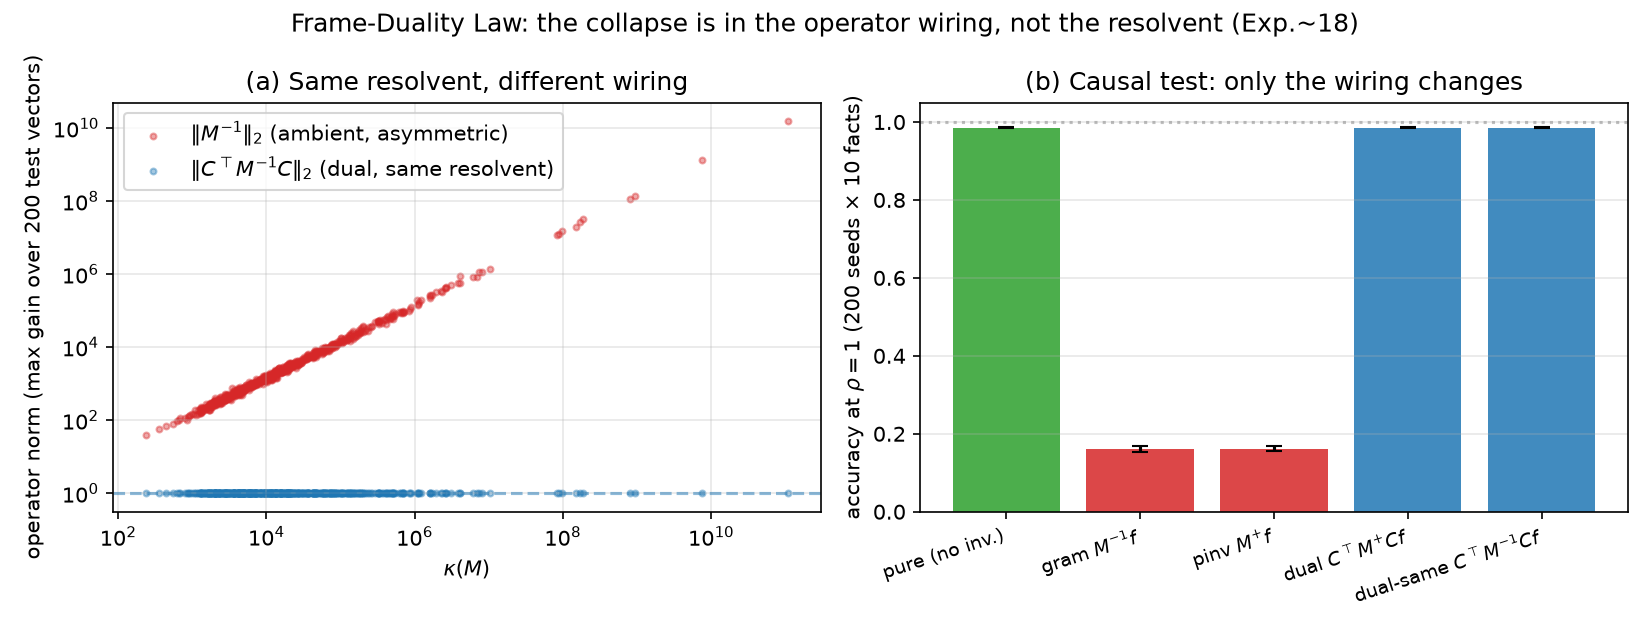
\includegraphics[width=\linewidth]{figures/fig_exp18_frame_duality.png}
  \caption{Exp.~18: decoding accuracy at $\rho=1$ (right) and the exact operator norms (left): $\|M^{-1}\|_2 = 1/\lambda_{\min}(M)$ (red) vs $\|C^{\top} M^{-1} C\|_2 = 1$ (blue). The collapse belongs to the placement. In the rank-deficient regime $\rho = 1.333$, \texttt{dual-same} with the un-truncated inverse drops (the operator is no longer a projector) while \texttt{dual} (pseudo-inverse) holds, as predicted by Obs.~\ref{obs:fdl}.}
  \label{fig:exp18}
\end{figure}

The control on feedback (Exp.~18, Section~12 of the protocol) separates loop dynamics from operator instability: at $T=1$ the pure resonator is already imperfect ($0.911$, it needs iterations to converge) while gram is already collapsed ($0.165$) --- the gram failure is present after a single application of $M^{-1}$, before any feedback. The loop is not what breaks gram; the operator placement is.

\begin{observation}[dual placement of spectral operators]
\label{obs:fdl}
Let $C \in \mathbb{R}^{n\times d}$ ($n$ codevectors in dimension $d$), $M = CC^{\top}$, and write the singular value decomposition $C = U\Sigma V^{\top}$. For any spectral operator $T = g(M)$ acting on the coefficient space $\mathbb{R}^{n}$,
\[
  C^{\top} T C \;=\; V \,\Sigma\, g(\Sigma^{2})\, \Sigma\, V^{\top},
\]
so its nonzero eigenvalues are $\sigma_i^{2} g(\sigma_i^{2})$ acting on the directions $V$, and $\|C^{\top} T C\|_2 = \max_i |\sigma_i^{2} g(\sigma_i^{2})|$. In particular:
(a) for $T = M^{-1}$ with $M$ invertible (square, $n=d$, full rank), $\sigma_i^{2}g(\sigma_i^2) = 1$ so $C^{\top} M^{-1} C = I$;
(b) for $T = M^{+}$, $\sigma_i^{2} g(\sigma_i^2) = 1$ on the spectrum and $0$ off --- a clean projector;
(c) for Tikhonov $T = (M + \alpha I)^{-1}$, $\sigma_i^{2}g(\sigma_i^2) = \sigma_i^{2}/(\sigma_i^{2} + \alpha) < 1$;
(d) for a truncated SVD, the same with $1$ on kept modes and $0$ on truncated.
Under ambient placement $T$ acts directly on the ambient state with $\|T\|_2$ unbounded as $\lambda_{\min} \to 0$; the dual placement $C^{\top} T C$ is bounded by $\|T\|$-weighted frame geometry and, for the projective operators, is exactly $\|P_{\operatorname{row}(C)}\|_2 = 1$.
\end{observation}

\paragraph{Attribution to classical frame theory.} Observation~\ref{obs:fdl} is a direct application of the canonical dual frame: for a frame $C$ with frame operator $S = C^{\top} C$, the canonical dual is $\tilde{C} = S^{-1} C^{\top}$, and the reconstruction $\tilde{C}^{\top} (\cdot)$ composed with the analysis $C$ yields the projector $C^{\top} (C C^{\top})^{+} C$ onto the row space \citep{duffin1952class, christensen2016introduction}. The case $T = M^{-1}$ at the square point is the elementary identity $C^{\top}(CC^{\top})^{-1}C = I$ for invertible square $C$. We state Obs.~\ref{obs:fdl} only to pin down \emph{which} operators neutralize in dual placement for the resonator setting (Exp.~23); we do not claim it as a new mathematical principle. The contribution of this paper is the identification of the hard-edge ambient-resolvent failure mode (Def.~\ref{def:closure}), its causal attribution to operator placement (Exp.~18), and the empirical verification of the classical repair across algebras and ensembles.

The observation is supported at four independent levels: (i) causal intervention with fixed codebook, Gram, resolvent, states, facts, and iterations (Exp.~18); (ii) a from-scratch reimplementation with no shared code (Exp.~19); (iii) transfer across six codebook ensembles, the BSC algebra, and a de-VSA-ified purely linear pipeline (Exps.~20, 18b, 21); and (iv) a perturbation analysis showing that the stabilization extends to $T = M^{+}$, Tikhonov, and truncated SVD (Exp.~23): the dual gain equals $1$ exactly for the projective constructions $M^{-1}$ and $M^{+}$, and sits slightly below $1$ for the regularized variants (Tikhonov, truncated SVD --- they shrink the weak eigendirection by design). A numerical bound on $\|C^{\top} T C\|_2$ relative to $\|T\|$ is measured in Exp.~26.

\textbf{Independent replication (Exp.~19)}. A from-scratch reimplementation (60 seeds, 5 initializations per codebook, no shared code with the main harness) recovers the same effect: \texttt{pure} $0.982$, \texttt{gram} $0.159$, \texttt{dual-same} $0.982$, paired per-seed $+0.823$ with $100\%$ of seeds positive.

\textbf{Ensemble generality (Exp.~20A)}. The same intervention across six codebook families at $\rho=1$: Gaussian ($0.160 \to 0.979$), Rademacher ($0.128 \to 0.986$), uniform-on-sphere ($0.164 \to 0.983$), and Toeplitz-correlated ($0.175 \to 0.947$) all replicate; an orthogonal frame (QR factor of a Gaussian matrix; for $n=d$ it satisfies $C^{\top}C=I$, so $M=I$ and ambient inversion is well-defined and harmless) provides a control: $\rho=1$ alone does not force the collapse --- the hard-edge geometry of a \emph{random} square Gram does; a trivially well-conditioned square Gram does not. A deliberately pathological near-duplicate frame breaks all decoders, as expected.

\textbf{Aspect-ratio sweep (Exp.~20B)}. On the Gaussian ensemble, the collapse is localized to the hard-edge region: ambient decoding is benign at $\rho \le 0.95$, collapses at $\rho = 1$ ($\kappa \sim 2.5\times 10^{3}$), and at $\rho > 1$ the Gram ceases to exist (rank-deficient) so the correction cannot be applied.

\textbf{De-VSA-ified linear probe (Exp.~21)}. Bypassing the resonator entirely with $f \mapsto \{$ambient vs.\ dual$\}\,(f+\epsilon)$: ambient gain $= 3.6\times 10^{2}$ median (p99 $1.3\times 10^{3}$), dual gain $= 1.000$ exactly. HRR/VSA was the delivery vehicle, not the cause.

\textbf{Iteration dynamics (Exp.~22)}. Tracking the error over $T=50$: the ambient decoder's error at $t=0$ is already $\approx 6.8\times 10^{3}$ (the initial estimate is random, so the first application of $M^{-1}$ blows it up) and stays there; the dual decoder starts at $1.66$ and converges to $0.92$. Growth-rate fit over the first ten iterations: $a_{\text{gram}} \approx 1.00$ (saturated noise floor), $a_{\text{dual}} \approx 0.97$ (converging). The loop is not the amplifier; the first application already destroys the ambient state.

\begin{figure}[t]
  \centering
  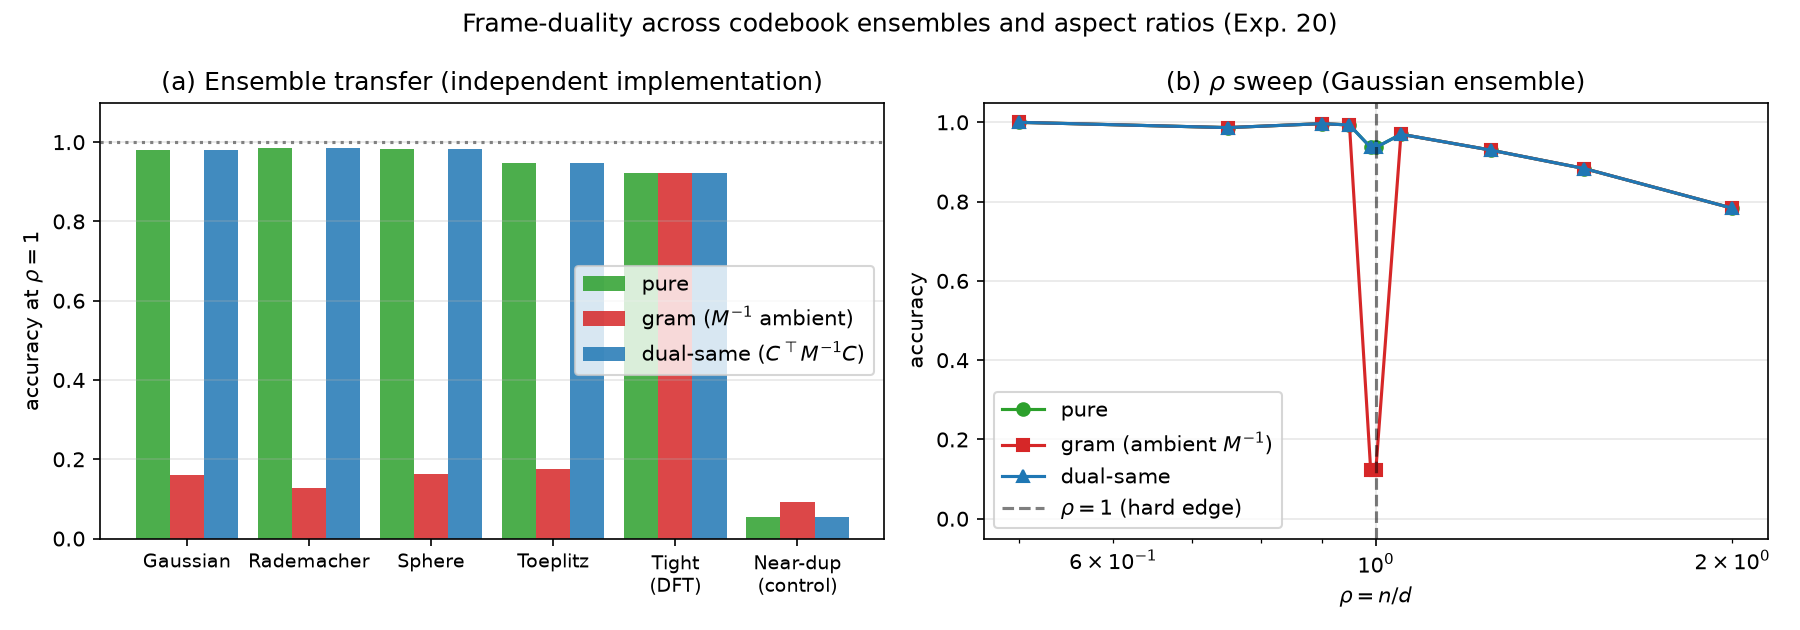
\includegraphics[width=\linewidth]{figures/fig_exp20_ensembles.png}
  \caption{(a) The placement effect transfers across codebook ensembles (Exp.~20A): ambient $M^{-1}$ collapses in Gaussian, Rademacher, uniform-sphere, and Toeplitz codebooks; the coefficient-space placement recovers decoding everywhere. Right panel: (b) the Gaussian $\rho$-sweep localizes the ambient collapse at the hard edge $\rho=1$.}
  \label{fig:ensembles}
\end{figure}

\textbf{Cross-algebra replication (Exp.~18b).} The same intervention in BSC (binary codevectors in $\{\pm 1\}^{d}$, bind = element-wise product), $100$ seeds $\times$ 10 facts at the square point: \texttt{gram} $0.192 \pm 0.011$, \texttt{dual-same} $0.995 \pm 0.002$ using the same resolvent, paired difference $+0.80$ ($99.8\%$ of 1000 paired facts positive).

\textbf{FHRR-complex replication (Exp.~27)}. Finally, the causal test in the original algebra: complex unit-modulus codevectors, Gram $M = C C^{H}$, dual $C^{H} M^{-1} C$. At the square point with the same protocol (60 seeds, 5 inits): \texttt{pure} $1.000$, \texttt{gram} $0.131$, \texttt{dual-same} $1.000$, paired $+0.868$ ($100\%$ positive). The effect closes the circle on the originating algebra: HRR, BSC, and FHRR all reproduce the ambient-collapse / dual-recovery signature.

\section{Failed Alternatives}
\label{sec:failed}

\paragraph{Gradient decoder.} Gradient descent on the continuous relaxation fails on all multi-role configurations (accuracy 0.08--0.33), regardless of $\rho$. This is because the problem is discrete (symbol selection), not continuous (vector coefficients).

\paragraph{Geometric parametrization.} Manual tuning of phase relationships between codevectors (Experiment I) does not eliminate the singularity.

\paragraph{Condition-number band as trigger.} Exp.~17 refutes the hypothesis that the collapse is triggered when $\kappa$ crosses a critical window: seeds with $\kappa$ as low as $2.3\times 10^{2}$ collapse identically to seeds with $\kappa \sim 10^{5}$. The trigger is the hard-edge geometry itself (Def.~\ref{def:closure}), not a scalar threshold.

\section{Discussion}
\label{sec:discussion}

The results identify a reproducible decoder failure mode at the square point and characterize its spectral mechanism: the ``binary collapse'' appears for ambient Gram-resolvent decoders exactly at $\rho=1$ (Def.~\ref{def:closure}), while the tested pure resonator and learned decoder remain accurate, and the classical coefficient-space repair restores decoding in the tested setup. Decoding behaviour in VSA therefore depends on the decoder class --- concretely, on where the decoder places its resolvent operators.

\subsection{Open problems and falsification agenda}

The operator-placement account was stated provisionally before this agenda; after running it, all planned falsification experiments support it.

\begin{enumerate}
\item \textbf{Independent replication} (DONE). Exp.~19 implements the test from scratch with a different codepath: pure $0.982$, gram $0.159$, dual-same $0.982$.
\item \textbf{Ensemble generalization} (DONE). Exp.~20A: Gaussian, Rademacher, uniform-sphere, Toeplitz all replicate; the orthogonal frame (square) does not collapse because $M=I$; near-duplicate breaks all. Exp.~20B: $\rho$ sweep localizes to the hard edge.
\item \textbf{Discrete aspect-ratio sweep} (DONE, within the Gaussian ensemble). Exp.~20B varies $d$ over integer values, giving distinct geometries per point; the collapse localizes to $\rho=1$.
\item \textbf{Perturbation amplification} (DONE). Exp.~21: ambient gain $3.6\times 10^{2}$ median, dual $=1.000$.
\item \textbf{De-VSA-ified linear pipeline} (DONE). Exp.~21 reproduces the dichotomy without a resonator.
\item \textbf{Operator zoo} (DONE). Exp.~23: $M^{+}$, Tikhonov ($\lambda=10^{-3}, 10^{-1}$), truncated SVD in both placements. The dual gain equals $1$ exactly for $M^{-1}$; for $M^{+}$ on well-conditioned inputs the dual gain is also $1$, while on a deliberately ill-conditioned Gram ($\kappa \sim 10^{11}$) the truncated SVD inside the pseudo-inverse yields a gain of $0.992$, correctly reflecting the projector's loss of the near-null eigendirection. Tikhonov sits below $1$ by design ($\sigma_i^2/(\sigma_i^2+\alpha)$).
\item \textbf{Iteration dynamics} (DONE). Exp.~22: ambient $e_0 \approx 7\times 10^{3}$ (saturates on first application), dual converges ($a < 1$).
\item \textbf{Counterexample search} (DONE). Exp.~25: deliberately constructed matrices (quasi-collinear down to $\epsilon=10^{-6}$, ill-scaled, block-diagonal, tall, wide) all confirm the pattern --- ambient diverges, dual stable; the wide case $n<d$ yields gain = $\sigma_{\max}(P_{\mathrm{row}(C)}) < 1$, matching the projector prediction.
\end{enumerate}

The connections to classical frame theory are direct: $C^{\top} M^{+} C$ is the canonical dual-frame projector \citep{duffin1952class}, and the operator placement question translates existing results on stable reconstruction \citep{eldar2018sampling} into the resonator-decoder setting. We view this as feature, not bug: the repair comes with 70 years of supporting theory.

\paragraph{Connection to capacity theory.} Our finding that $\rho = 1$ is a point singularity complements capacity analyses \citep{thomas2023capacity} that focus on asymptotic scaling. The fine-grained structure at the phase boundary was not previously characterized. Through the Wishart lens (Sec.~\ref{sec:rmt}), the $\rho$ axis is exactly the aspect-ratio axis of the Marchenko--Pastur law \citep{marchenko1967distribution}, and the singular point corresponds to the soft-edge-to-hard-edge crossover of the square ensemble \citep{tracy1994level, edelman1988eigenvalues}.

\paragraph{Connection to transformers.} The residual stream of transformers can be interpreted as a VSA \citep{dhayalkar2025binding}. Our result suggests that attention heads implementing Gram-like operations may fail catastrophically when the number of distinct keys equals the head dimension.

\paragraph{Limitations.} The operator-placement account is supported by independent reimplementation (Exp.~19), six codebook ensembles with pathological controls (Exp.~20, Exp.~25), BSC (Exp.~18b), FHRR (Exp.~27), a purely linear pipeline (Exp.~21), dynamics (Exp.~22), the operator zoo (Exp.~23), exact frame-bounds controls (Exp.~24), and a naive stability bound measured against its slack (Exp.~26). Open: (i) a proof of the bound for non-spectral-frame $T$; (ii) FHRR beyond the square point; (iii) asymptotic confirmation of the $\kappa \sim 4n^{2}$ slope at $n \gg 512$, since the current evidence is at finite sizes with heavy-tailed spread; (iv) the main harness's ambient correction is dimensionally applicable only at $\rho=1$, so the away-from-square behavior of the ambient decoder is characterized by the coefficient-space (Exp.~11c) and linear-pipeline (Exp.~21) controls rather than by the ambient resonator itself.

\section{Conclusion}
\label{sec:conclusion}

The experiments identify a reproducible square-point failure in the tested resonator configurations and characterize its spectral mechanism. The ``binary collapse'' is decoder-relative: it appears for Gram-resolvent decoders applied to the ambient state exactly at $\rho=1$ (Def.~\ref{def:closure}). The tested pure resonator and learned decoder remain accurate, and the canonical dual-frame projector --- classical mathematics --- repairs it completely. VSA design should therefore focus on operator placement, not just representation capacity --- and the reported failure mode is diagnosable a priori from the codebook aspect ratio and the decoder's operator structure.

\section*{Data availability}

All code, raw data, and figure scripts are available at \url{https://github.com/Rylow999/fhrr-rho-collapse}. Each number in the text is traceable to a file under \texttt{data/}; experiments are seeded and listed in \texttt{src/} (\texttt{exp\_V9\_fine\_rho}, \texttt{exp\_V14\_kappa\_law}, \texttt{exp\_V16\_scaling\_n}, \texttt{exp\_V17\_kappa\_vs\_acc}, \texttt{exp\_V11b/11c}, among others). The verification script described in the text reproduces every headline number from the shipped JSON files, and the central algebraic claim is covered by unit tests (\texttt{tests/test\_frame\_duality.py}) run in continuous integration.

\section*{Acknowledgments}

The author thanks the anonymous external reviewer whose critique of the $\kappa$-band claim led to the current, stronger formulation, and a second reviewer whose insistence on distinguishing the failure mode from the representation sharpened the framing of this revision.

\bibliographystyle{plainnat}
\bibliography{references}

\end{document}
